\chapter{Marco Teórico}

 En este capitulo se aborda el marco teórico necesario para comprender mas fácilmente el desarrollo de los capítulos posteriores. Se analiza el problema del trafico en general, los simuladores y la teoría detrás del algoritmo a utilizar.

\subsection{Problema del transito vehicular}

En gran parte del mundo se esta produciendo un crecimiento sostenido del parque automotor lo que ocasiona una serie de problemas que afectan la calidad de vida de las personas relacionados con el agravamiento de las congestiones vehiculares \citep{Cepal2003}.

Este problema tiene un impacto grande en el desarrollo de las ciudades por lo que es un componente principal en los planes estratégicos para su crecimiento.

La congestión ocasiona una progresiva merma en la velocidad promedio de circulación, lo que incrementa la duración de los viajes, aumenta el consumo de combustible y la contaminación atmosférica y sonora, lo que repercute directamente en la salud de las personas. 
Ademas se genera una exigencia en las vías de transito que ocasiona un deterioro mayor de calles y rutas.

Uruguay no escapa a este fenómeno en particular Montevideo, donde el aumento del parque automotor esta en ascenso constante desde el 2005 \citep{INE2014} 
Y según proyecciones el crecimiento seguiría en un promedio de 4.5\% anual hasta el 2020. \citep{BBVA2013}

Esto viene de la mano con el sostenido aumento de las ventas de vehículos  desde el 2003 \citep{Autoanuario2014}

Los expertos indican que la congestión ya esta instalada y la infraestructura vial no acompaso este crecimiento. Ademas se indica que Montevideo es la ciudad con mas semáforos por automóvil en Latinoamerica. Con mas de 620 cruces semaforizados, alguno de los cuales no estan coordinados.\citep{Subrayado2013}

Por todo esto relevante el tema de la sincronización de semáforos para agilizar el transito y no generar congestiones, aumentando la velocidad promedio de los viajes y mejorando las perspectivas de desarrollo de la ciudad asi como la calidad de vida de sus habitantes.

\subsection{Corredor Garzón}
El corredor Garzón esta ubicado en Montevideo Uruguay, fue construido como parte de un plan de movilidad que incluye otros 4 corredores. 
Presenta un carril exclusivo para ómnibus y preferenciales
http://www.montevideo.gub.uy/ciudadania/stm-transporte-metropolitano/plan-de-movilidad/corredores

Tiene 6km de largo , extendiéndose desde ...  hasta ..
%http://www.montevideo.gub.uy/sites/default/files/articulo/corredor_garzon.pdf

Agregar mapa

Los problemas de sincronización de semáforos fueron admitidos en varias publicaciones.

18 diciembre 2013 - Corredor Garzón lucha contra el tiempo %http://www.elpais.com.uy/informacion/imm-corredor-garzon-tiempos-cambios.html
Dice que antes de Garzon se demoraba promedio 18 minutos, y al inaugurar el corredor 30 minutos. Después se mejoro algo para equilibrar los tiempos
Para el jerarca, eso se dio "con la diferencia de que hoy hay 15 semáforos más y se ganó en seguridad". En concreto, tras la obra, se pasó de tener 5 semáforos a 20. Según Campal, su des-coordinación inicial, entre otros aspectos, fue lo que provocó tales demoras, generando malestar en los usuarios.
inversión de 60 millones


4 agosto 2013 - Garzon desde un omnibus %http://www.elpais.com.uy/informacion/corredor-garzon-visto-bus.html


30 julio 2013  - Intendetnta admite errores %http://www.elpais.com.uy/informacion/garzon-olivera-admitio-errores.html
La intendenta admte errores y dice: no se ha logrado sincronizar los semáforos. Hay un tema con el software,(y) la empresa subcontratada no ha dado los resultados esperados


Abril 2013 - Otro Corredor con obras paralizadas por criticas a GArzon
%http://www.elpais.com.uy/informacion/marcha-atras-en-corredor-agraciada.html





\section{Algoritmos Evolutivos}
Los algoritmos evolutivos son métodos no determinísticos que se inspiran en la evolución natural de las especies utilizando conceptos como población, cruzamiento, mutación, selección, etc. Estos se utilizan para resolver problemas de optimización y búsqueda, entre otros. []

Es una técnica iterativa que busca en cada paso mejorar las soluciones por medio de operadores y basado en un criterio predefinido para maximizar o minimizar.

Este tipo de solución a demostrado su utilidad en una amplia variedad de problemas complejos.


\subsection{Algoritmos Genéticos}
Un algoritmo genético es un tipo de algoritmo evolutivo, siendo de los mas populares.

La idea base es que partiendo de una población inicial de individuos se seleccionan los mejores en base a su aptitud respecto a solucionar el problema y estos se utilizan para generar nuevos individuos ya sea por combinación o modificación. Por tanto en cada paso obtenemos mejores soluciones hasta detenernos usando un criterio de parada ya sea el numero de iteraciones o cuando ya no se puede mejorar mas la solución.

Un individuo es una codificación de la solución que resuelve el problema.
La población inicial puede generarse aleatoriamente o basándose en algún conocimiento previo.
La función de evaluación indica que tan buena o apta es una solución en comparación con las demás.
En cada iteración la cual se llama generación se aplican operadores de cruzamiento estos son formas de combinar a los individuos para obtener otros que potencialmente sean una mejor solución y también cambios aleatorios sobre los individuos llamado mutación.

Por tanto se van seleccionando, combinando y cambiando las mejores soluciones en un proceso que va obteniendo mejores soluciones.
El criterio de parada nos indica cuando termina este proceso, ya sea por que se alcanzo un numero de generaciones predefinidos o por que la mejora no es tan evidente. Al final se devuelve la mejor solución encontrada en todo el proceso.


Hay que indicar que no es una técnica exacta pero si logra muy buenas aproximaciones y es muy buena en problemas complejos por su flexibilidad y robustez. 


\subsubsection{Representación de soluciones}
No podemos trabajar directamente sobre las soluciones, por lo que tenemos que codificarlas en un modelo que nos sirva para poder aplicar el algoritmo.
La inspiración biológica se ve en los nombres que adopta esta representación, llamada Cromosoma que es un vector de genes y cada valor de un gen se llama alelo.
En general se codifica un vector de números binarios o reales de largo fijo, lo que facilita la aplicación de los operadores.

\subsubsection{Función de Evaluación} 
Indica que tan bueno es un individuo para resolver el problema en cuestión con un valor conocido como Fitness. Este se utiliza para seleccionar a los mejores y de esta forma guiar la exploración hacia la mejor solución.
Se deben tener en cuenta las restricciones del problema para que las soluciones no factibles no sobrevivan.
En general es donde se consume el mayor tiempo del algoritmo en comparación con los demás operadores.

\subsubsection{Operador de Selección}
Existen diversos operadores de selección , su función es que las mejores características de los individuos se mantengan en las siguientes generaciones.
Ruleta:
Torneo:
Elitismo:

\subsubsection{Cruzamiento}
Su función es combinar individuos para lograr mejores soluciones. 
Existe una taza que se puede modificar para indicar la probabilidad de que se realice el cruzamiento.
Cruzamiento de un punto:
Cruzamiento azar

\subsubsection{Mutación} 
Indica el método utilizado para modificar un individuo, esto se realiza para lograr mas diversidad y no caer en máximos locales. En general aplica una modificación aleatoria en el cromosoma.
También hay una taza de probabilidad, en general es baja.

\subsubsection{Reemplazo} 
Se indica cual es el criterio que debemos tomar para crear una nueva población, ya sea tomando solo los nuevo hijos creados, comparando también con los padres o aplicando algún otro criterio.

\subsubsection{Criterio de parada} 
Indica cuando debe terminar el algoritmo, puede ser definiendo un numero fijo de generaciones o analizando si la mejora en soluciones se estanco.

\subsection{Algoritmos Genético Simple}

El algoritmo que vamos a utilizar es el simple, propuesto por Goldberg [] 
El operador principal es el de cruzamiento y el secundario la mutación.

Su esquema de funcionamiento es el siguiente


\begin{algorithm}%[!ht]
	\caption{Algoritmo Genético Simple}
	\label{alg:algoritmo_genetico_simple}
	\begin{algorithmic} [1] 
		{
			%\small
			\STATE {Inicializo( Pob(0))}
			\STATE \texttt{generacion} = 0
			\WHILE {\text{No llegue al criterio de parada}}
			\STATE {Evaluar Pob(generacion)}
			\STATE {Padres = Seleccionar(Pob(generacion))}
			\STATE {Hijos = Cruzamiento(Padres) y Mutacion(Padres)}
			\STATE {NuevaPob = Reemplazar Pob(generacion) con Hijos}
			\STATE \texttt{generacion}++
			\ENDWHILE
			\RETURN Mejor solución
		}
	\end{algorithmic}
\end{algorithm}




\subsection{Algoritmos genético multiobjetivo}



En este caso se busca una solución que satisfaga de forma simultanea las restricciones y varios objetivos diferentes.

\subsubsection{Por que elegimos multiobjetivo?}
La intendencia apoya el cambio del trafico en la ciudad de Montevideo para que se haga mayor uso del transporte urbano[] y disminuir la cantidad de automóviles circulantes para disminuir el trafico y la contaminación. En este sentido se da prioridad a los ómnibus, por esta razón nuestro algoritmo puede varían los diferentes pesos para dar mas prioridad a la velocidad promedio de ómnibus vs el resto de los vehículos.
 
Se busca que la gente prefiera el ómnibus, uno de los factores es la duración del viaje, si se logra mejorar esto se estaría cumpliendo uno de los objetivos de la intendencia
SUMO brinda mucha información referente a los viajes, por lo que tenemos varias métricas a elegir para nuestro algoritmo. Entre ellas se destacan: Cantidad de vehículos que llegaron a destino, Tiempo de viaje promedio, Tiempo de ocupación promedio, velocidad promedio global, tiempo parado q emite gases. Decidimos usar la velocidad promedio separando entre ómnibus y autos. De esta forma podemos optimizar ambos en el sentido multiobjetivo, o priorizar uno sobre el otro.


\subsection{Algoritmo Genético Paralelo}
Los problemas complejos suelen requerir una alta demanda computacional por lo que aplicar técnicas de paralelización es útil para lograr tiempos de ejecución menores.

Existen varios niveles de paralelización ya sea a nivel global enfocándonos en paralizar la función fitness, a nivel de la población, o a nivel del individuo. \citep{Nesmachnow2002}

En el caso de los algoritmos genéticos gran parte del tiempo se realiza en la etapa de evaluación , cerca de un 90 \% del tiempo[]
Por esta razón es una forma buena de distribuir la carga en varios procesadores para que las evaluaciones se realicen en paralelo.


\subsection{Maestro-Esclavo}

En este modelo un proceso maestro es el encargado de realizar los operadores básicos del algoritmo y distribuir a procesos esclavos la evaluación de la función fitness para un conjunto de individuos, el esclavo devuelven el resultado y luego el maestro es el encargado de continuar ejecutando los operadores.

De este modo aumenta la eficiencia computacional del algoritmo ya que una de las funciones mas costosas es distribuida entre varios nodos.

\begin{figure}[H]
\centering
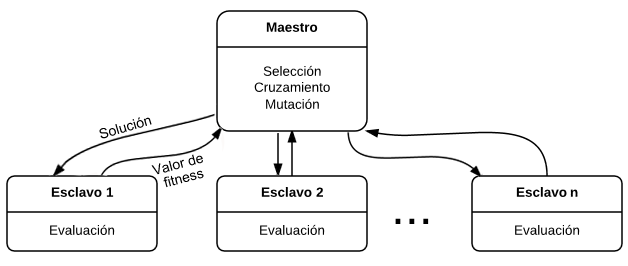
\includegraphics[width=0.7\linewidth]{Figures/diagrama-master-slave}
\caption[Modelo Maestro-Esclavo]{Modelo Maestro-Esclavo}
\label{fig:diagrama-master-slave}
\end{figure}



\subsection{Resumen}




\section{Simulación y herramientas}

\subsection{Simuladores de trafico}
Los simuladores de trafico son programas que simulan el movimiento de vehículos sobre una red de calles,es una herramienta muy usada en la investigación de trafico vehicular, así como estudio de congestiones o análisis de impacto que tendrán nuevas infraestructuras.  Las razones para usar una simulación son varias, entre ellas se encuentra  la rapidez  ya que la simulación se puede realizar en tiempo mucho mas rápidos que en la realidad, el costo en dinero ya que no estamos afectando el escenario real  y tampoco tenemos que modificar o detener el escenario real para probar nuevos parámetros. Ademas nos sirve para poder prever situaciones que podrían darse bajo determinadas circunstancias.

Los simuladores se pueden dividir en microscópicos o macroscópicos según el nivel de detalle de la simulación. Un simulador macroscópico modela  el trafico vehicular como un fluido. En cambio un simulador microscópico simula el movimiento de cada vehículo según sus características particulares.
SUMO es uno de los simuladores abiertos mas populares,  es microscópico aunque presenta algunas dificultades a la hora de la configuración del mapa y el transito que lo hace en base a archivos XML.

Cuanto mas crece el numero de vehículos y la complejidad de la red de mapas mas difícil se hace crear la entrada básica que necesita el simulador. Aunque existen diversas herramientas que ayudan a este proceso aun se requiere un trabajo manual para el acondicionado de estos archivos.
SUMO simula el trafico utilizando archivos XML que representan las rutas, los vehículos y el trafico. En 

\subsection{Modelo de trafico }
Esta es la representación de la circulación de vehículos, existen varios métodos desde 
Aleatorios: Genera diferentes recorridos que seguirán los vehículos aleatoriamente
JTR : basados en probabilidades en los cruces  es decir cuando un vehículo llega a un cruce tiene cierta probabilidad de seguir o doblar (JTR – junction turning ratio), 
Basado en distritos:  Se especifican distritos(conjunto de calles) y  la cantidad de movimiento vehicular entre ellos en una  matriz
Basado en Actividad: Se especifica la cantidad de casas , vehículos y población en un determinado lugar y el modelo genera la densidad de trafico que se producirá basado en los tipos de actividades que se realizan comúnmente como ir al trabajo, hacer las compras, ir a la escuela,  etc
Definido por el usuario: que permiten determinar la ruta de los vehículos con mayor detalle.

\subsection{Representaciones}

\subsubsection{Red calles}
La red de calles se representa como un gráfico dirigido en un archivo xml con extensión .net.xml . Alli se especifican los nodos, y vértices así como sus atributos. También se representan los semáforos. Esto  se genera utilizando una herramienta  para convertir un mapa al formato que SUMO utiliza.

\subsubsection{Representación Trafico}
En este caso también se utiliza un archivo xml donde se definen las rutas y los trips. Un trip representa el movimiento de un vehículo de un punto inicial hacia un punto final (El recorrido se hacen en tiempo de ejecución utilizando el camino mas corto basado en el trafico). Una ruta es mas complejo que un trip ya que agrega todos los vértices por los que el vehículo pasara.

SUMO también soporta el modelo JTR y basado en distritos pero se necesitan módulos externos para generarlos.

\subsubsection{Representación del tiempo}
El tiempo se representa como una serie de pasos discretos, cada uno durando un segundo. Este valor se puede modificar aunque es recomendado dejarlo así para que sea consistente.

\subsection{Trafico}
Elegimos utilizar el flow calle-a-calle que nos permite determinar con mucho detalle el trafico generado entre calles. Ya que contamos con datos relevados en el lugar. Se especifica el lugar de donde sale el vehículo, donde termina su recorrido, el numero de vehículos que se emiten o la frecuencia.

\subsubsection{Tipos de vehículos}
Se pueden crear diferentes tipos de vehículos especificando propiedades como largo, velocidad máxima,  aceleración, color, etc. También contamos con algunos por defecto como camiones, buses

\subsubsection{Accidentes}
El simulador permite representar colisiones y el corte de una calle. Decidimos no utilizar esto pues no queríamos este tipo de variables afectara en la ejecución de las pruebas.

\subsection{Trabajo de campo realizado}
Al no contar con datos públicos sobre la configuración de los semáforos de la zona, realizamos un revelamiento in-situ de la siguiente forma.
En los principales cruces realizamos una filmación de 30 min. Luego analizamos el vídeo realizando el conteo manualmente con la posibilidad de enlentecer el vídeo para mayor facilidad.
Estas medidas nos sirvieron para verificar nuestros modelos basados en los datos del GPS 

La configuración de los semáforos se realizo yendo por el corredor y cronometrando la duración del tiempo. Tanto en ida como en venida para coproborar que fueran correctos.



\subsection{Configuración de la simulación}


Generar un mapa compatible con el simulador de transito mejor al que tenemos del año pasado con los últimos detalles del corredor.

Edicion del mapa http://fmachado.dei.uc.pt/wp-content/papercite-data/pdf/misc13.pdf pequeño articulo sobre sumo, mismas dificultades que tuvimos el año pasado esperemos que las mejoras del netconvert hayan sido buenas sino vamos a estar un buen rato tocando xml

Creación del modelo del trafico
	Obtención de datos: Tuvimos reuniones con la IMM que con muy buena disposición nos aporto datos relativos a la posición de los ómnibus?
	Con los datos realizamos un modelo vehicular de la ciudad [poner el mapa] que nos da una noción básica sobre el trafico en ciertos puntos de la ciudad, y la velocidad promedio de circulación.
	este modelo luego fue validado con revelamiento in-situ de diferentes puntos.

Tener en cuenta los cambios en el corredor:
	Buscar información publica sobre las luces- no hay- tomar medidas 
	Actualmente no se cuenta con información publica relativa a la configuración de los semáforos en la ciudad, aunque cabe destacar que en el futuro se prevé crear un sistema centralizado de sincronización de semáforos.  [http://www.elobservador.com.uy/noticia/292066/imm-sincronizara-400-semaforos-para-agilizar-el-transito-capitalino/] 
	buscar info sobre densidad - no hay- contar
	Cantidad de luces por semáforo
	Realizar nuevas mediciones de tiempos de luces
	Densidad del trafico actual (se puede conseguir o tomar mediciones)
	bondis: frecencias de bondis
	de donde sacamos esta info?
	autos: .py genera aleatorio


\subsubsection{Diseño del mapa}
El mapa base de la zona lo tomamos de OSM, luego se cotejo su exactitud con Google Maps y Bing Maps.
Utilizamos la herramienta netconvert para pasarlo a formato que SUMO acepte. 
Para esto realizamos varios ajustes editando los archivos xml para indicar donde se realizan.

Se generó una especial dificultad en el diseño de un mapa que
fuese tan fiel como fuese posible a la realidad y que también
fuese compatible para usar con  Sumo. Se debió recabar datos
in  situ  ya  que  hasta  la  misma  intendencia  [4]  tenía  errores
respecto a la realidad, falta de algunos semáforos, etc. Luego al
pasarlo  al  formato  compatible  con  sumo  se  debieron  corregir
calles,  cruces  y  todas las  posibles  conexiones de  las  esquinas
del corredor que debieron ser escritas a mano en un XML.

Poner fotos de un ants (salida directa del netconvert) y luego con los agregados de joins y connections


\subsubsection{Vehículos}
Se manejaron dos tipos de vehículos, autos y ómnibus:
Las  líneas  de  ómnibus  urbanas  (que  circulan  por  el
corredor)  incluidas  fueron  la  “G”,  la  “409”  y
adaptaciones  de  la  “522”  y  “148”  que  se  juntaron  en
una  línea  sola. Y  las líneas de ómnibus suburbanas en
el  tramo  elegido  realizan  el  mismo  trayecto  y  les
llamamos  línea  “A".  Todas  las  líneas  de  ómnibus
fueron cargadas con las paradas correspondientes y se
hicieron  variantes  en  los  viajes  dentro  de  una  misma
línea de manera que no siempre paran en los mismos
lugares.
Los  viajes  de  los  autos  son  generados  aleatoriamente
de modo que no circulen por el corredor (que es para
los  ómnibus  urbanos)  y  de  forma  que  tengan  mayor
probabilidad los viajes que comienzan y terminan en el
borde  de  la  red,  luego  se  seleccionan  los  viajes  de
manera  que  las  grandes  avenidas  sean  más  recorridas
que  las  calles  menos  importantes.

\subsubsection{Semáforos en cada cruce}
Se  tomaron  los  tiempos  de  cada  luz  de  los  semáforos  en
cada  cruce  y  luego  estos  datos  fueron  cargados  al  simulador
para comparar con los  resultados  así como también para base
de nuestro algoritmo evolutivo.

\subsubsection{Escenarios}



\section{Herramientas}

\subsection{Open Street Map:} 
http://www.openstreetmap.org/about  Es un proyecto en donde una comunidad crea mapas libres y editables. Cuenta con cerca de 1.8 millones de usuarios  y  mas de 20.000 que editaron algo en el ultimo mes [http://osmstats.neis-one.org/] por lo que es muy activa. Se utilizan datos de GPS móviles, fotografías satelitales y otras fuentes libres para crear los mapas y editarlos. 

\subsection{SUMO ( Simulation of Urban MObility)}
%http://sumo.dlr.de/wiki/Main_Page 
Es un simulador de trafico gratis y abierto que nos permite modelar redes de calles, vehículos, transporte publico, ciudadanos y semáforos. Sigue un modelo microscópico ya que realiza la simulación individual explicita de cada elemento. Ademas incluye un conjunto de herramientas destinadas  a facilitar la generación de trafico, construcción de mapas, etc. 


\subsection{Por que usar SUMO? }
otras alternativas? REvisar estado del arte?
Sumo es gratis
Nos permite utilizarlo sin interfaz gráfica por linea de comando lo que aumenta sensiblemente la velocidad ed ejecución, y  nos permite visualizar la interfaz gráfica una vez completada la optimización para ver exactamente como se comporta el sistema en la simulación.

Sumo presenta varias salidas con información interesante: http://sumo.dlr.de/wiki/Simulation/Output 
La salida obtenemos el tiempo de simulación, la cantidad de emitidos y la cantidad de completados. Buscamos que sea > 80%
Permite la ejecución tanto por linea de comando como una interfaz gráfica para visualizar

\subsection{NetConvert}
Utilizado para la generación de la red a partir de un mapa. Por ejemplo podemos transformar un mapa de openStreetMap a archivo XML de red que sumo reconoce.

\subsection{DUaRouter}
 Genera recorridos de vehículos basado en dinámicas definidas por el usuario.



\section{Resumen}

